\section{Marco Civil da Internet}
Com relação à ferramenta de consulta da Regulamentação do \mc, ela se apresenta como uma ferramenta bem mais completa que a anterior. Alguns ajustes visuais poderiam melhorar sua usabilidade – mas estes não são o foco do presente trabalho. Em termos de recursos, vislumbram-se duas possíveis melhorias que poderiam aumentar a participação.

\subsection{Comentários em ``sanfona''}
A primeira delas seria mostrar os comentários das pautas na página de listagem de pautas, sem que fosse necessário o usuário mudar de página. Na Figura \ref{fig:pautas-mcivil-hj} apresenta-se a página com a listagem de todas as pautas correntes. Nela podemos observar que o número de comentários de cada pauta está apresentado, porém para ver o comentário é preciso navegar até a página da pauta. Seria interessante que a visualização dos comentários (e a adição de novos) pudesse ser realizada na própria página de listagem de pauta, num fluxo similar ao fluxo do plugin wp-side-comments utilizado na consulta do anteprojeto de lei de proteção de dados pessoais.
    \begin{figure}[htb]%
        \begin{center}
            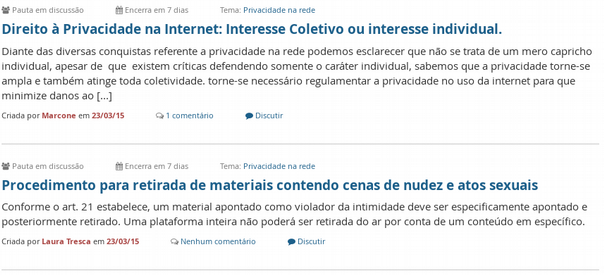
\includegraphics[scale=0.7]{./imagens/mcivil-atual-listagem.png}%
        \end{center}%
        \caption{Versão autal da listagem de pautas na consulta do \mc \label{fig:pautas-mcivil-hj}}%
        \fonte{Autoria Própria}%
    \end{figure}%
    
\subsection{Concordar / Discordar}
A segunda modificação seria a implementação do recurso ``concordar/discordar'' na própria pauta, não apenas nos comentários da mesma como é hoje, conforme pode ser observado na Figura \ref{fig:pauta-espec-mcivil}. De maneira análoga ao que foi proposto anteriormente, seria interessante após o voto de ``acordo'' ou ``desacordo'' convidar o usuário a explicar os motivos pelos quais ele concordou ou discordou do comentário e/ou da pauta.
    \begin{figure}[htb]%
        \begin{center}
            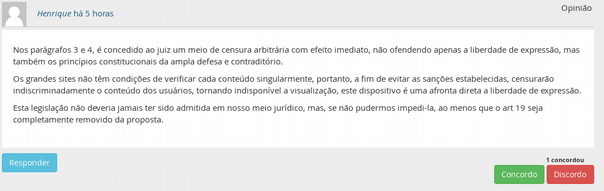
\includegraphics[scale=0.7]{./imagens/mcivil-comentario-pauta.png}%
        \end{center}%
        \caption{Comentário de uma Pauta específica \label{fig:pauta-espec-mcivil}}%
        \fonte{Autoria Própria}%
    \end{figure}%

\subsection{Redes Sociais}
	Se faz também necessária a implementação de recurso de compartilhamento de pautas/comentários/temas nas redes sociais, para que se possa atingir um público maior e aumentar as chances de colaboração. Este compartilhamento pode-se dar em alguns instantes distintos.
	
	O primeiro deles é simplesmente compartilhar uma pauta inserida por outrém. Este recurso está disponível, mas apenas dentro da página da pauta, quando ele poderia estar disponível na página de listagem de pautas também. Além disso, ele precisa ficar mais evidente. Conforme pode-se observar nas Figuras \ref{fig:pauta-espec-mcivil-share-comentario-fechado} e \ref{fig:pauta-espec-mcivil-share-comentario-ativo}, não está claro que existe a possibilidade de compartilhamento da pauta enquanto um recurso de rede social. Talvez a simples mudança na simbologia utilizada seja o suficiente neste caso, mas a mudança do posicionamento, alinhando o botão de compartilhamento com o título da pauta também pode ajudar.
    \begin{figure}[htb]%
        \begin{center}
            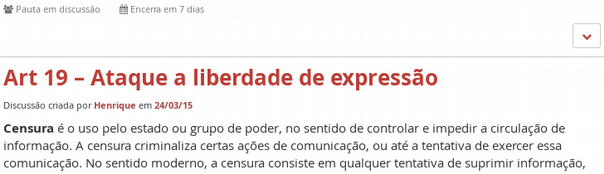
\includegraphics[scale=0.7]{./imagens/mcivil-social-share-01.png}%
        \end{center}%
        \caption{Página de uma pauta específica – Botão de compartilhamento quase escondido \label{fig:pauta-espec-mcivil-share-comentario-fechado}}%
        \fonte{Autoria Própria}%
    \end{figure}%
    \begin{figure}[htb]%
        \begin{center}
            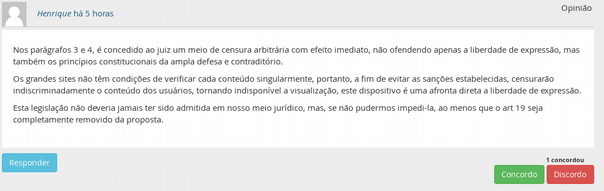
\includegraphics[scale=0.7]{./imagens/mcivil-comentario-pauta.png}%
        \end{center}%
        \caption{Página de pauta específica - Botão de compartilhamento ativo \label{fig:pauta-espec-mcivil-share-comentario-ativo}}%
        \fonte{Autoria Própria}%
    \end{figure}%
	Outro momento em que a opção de compartilhamento deveria ser apresentada aos usuários é ao inserir uma nova pauta, publicando-a no sistema e nas redes sociais simultâneamente.
	
	Por fim, ao adicionar um novo comentário (ou voto) numa pauta também deveria ser apresentada a opção de compartilhar o comentário (ou voto) nas redes sociais do usuário.

	Todas estas modificações seriam feitas no plugin “delibera” atualmente em uso na referida consulta.

\subsection{Pautas em destaque}
Para tentar fomentar ainda mais os debates, pode ser útil oferecer aos usuários a possibilidade de ver quais são as pautas mais debatidas, e talvez mais ``polêmicas''. Para isso existem duas possibilidades.

	A primeira delas é permitir reordenar as pautas pelo número de comentários (ou votos).

	A segunda delas é a utilização de ``marcadores'' de destaque. Pode-se pensar em ícones como o apresentado na Figura \ref{fig:mcivil-icone-pauta-destaque}, dentre outros.
	    \begin{figure}[htb]%
        \begin{center}
            
\includegraphics[scale=0.7]{./imagens/hot-topic.png}%
        \end{center}%
        \caption{Ícone de marcação de pauta em destaque \label{fig:mcivil-icone-pauta-destaque}}%
        \fonte{Autoria Própria}%
    \end{figure}%

\subsection{Ordenamento de pautas}
Visando facilitar a colaboração de usuários mais engajados, além de auxiliar em sistematizações, seria importante permitir também a ordenação das pautas por diversos critérios, sendo os principais:
\begin{itemize}
\item Quantidade de comentários;
\item Data de postagem;
\item Últimos comentários;
\item Quantidade de votos "concordo"; e
\item Quantidade de votos "discordo".
\end{itemize}

Desta forma os usuários mais ativos na plataforma podem encontrar de forma mais fácil os itens que possuem mais atividade, ou mais atividades recentes, sem precisar passar por todas as postagens.

O mesmo vale para a equipe que ficará responsável pela organização/sistematização da consulta, que poderá, ao longo do processo, acompanhar o desenvolvimento da consulta e, ao final, realizar destaques de forma simplificada.